\subsection{Procedure}
Here, the procedure of the test is explained in detail. 
The general data from the test, the description of the test course and the specified guidelines for the interview and observations of the test persons will be presented in the following sub-chapters.


General data about the test is seen here below, such as amount of participants, time and placement:
\begin{table}[!htb]
\begin{tabular}{l l}
Amount of participants: & 12 participants.\\
 & \\
Test subject data: & Convenience sampling: Aalborg university students.\\
 & \\
Estimated length of test: & 15-20 minute per test subject.\\
 & \\
Test location: & Aalborg University, conference room.\\
 & \\
Date of test: & 10/12 – 2013\\
 & \\
Estimated time of day: & 13:00 – 16:00\\
\end{tabular}
\end{table}


\subsubsection{Procedure: Test setup}
In the test setup, four persons were present for each test, i.e. 1 test subject, 2 observers and one person assisting the test subject. 
The test subject was placed on a chair with a laptop on a table in front of him/her. 
The webcam on the laptop was pointing towards the test subject, such that it would capture the gestures performed by the test subject while the test subject would also be able to see what was happening on the screen. 
At figure \ref{fig:testsetup} an illustration of the placement of the two observers can be seen. The two observers were placed slightly behind and to the side of the test subject to prevent any influence on the test subject by the observers. 
The observers were placed by a table with an assisting laptop and papers for notation. 
During the execution of the tests for each test subject, the assistant of the test subject would stay in the background, when not needed, in order to also prevent any influence on the subject.

\begin{figure}[!htbp]
\centering
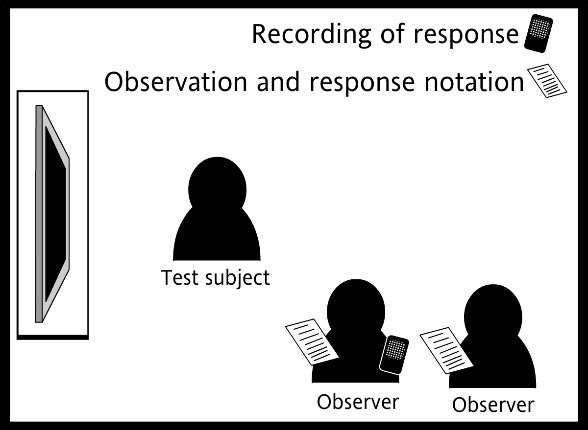
\includegraphics[scale=1]{Procedure1}
\caption{Test phase description} \label{fig:testsetup}
\end{figure}

Other individuals, such as subjects waiting for their turn to be tested and spectators, presented during the testing of one subject, were placed further away in the background, to prevent them from getting in the way.


\subsubsection{Procedure: Test materials}
A listing of all materials used during testing of all test subjects is presented here. 
This list excludes materials such as tables and chairs:
\begin{itemize}
\item Two laptops – one used by the test subject to play with the controllers and one for recording and noting observations (will be explained in the subchapter Test execution (\ref{sec:testexecution}))
\item The prototype controller described in the implementation (chapter \ref{sec:implementation})
\item Xbox 360 (SOTA) controller compatible with pc.
\item Notation paper-sheets – This includes blank papers for observations and papers with guidelines for the interview of the test subject (see Appendix \ref{app:questions} for interview guidelines)

\end{itemize}

This list includes all materials used by the test subject and/or the two observers described above. 
To elaborate on the prototype controller, it includes both the wheel-like controller and not the yellow sponge as the functionality of gear shifting was removed (described in usability test chapter \ref{sec:usability}).

\subsubsection{Procedure: Test execution} \label{sec:testexecution}
The test execution itself is parted into sequences, one for each test subject. 
Every test subject going through a testing sequence did the same things, but one difference between each half of the test subjects, was the order in which they went through the parts of the sequence.


Taking a starting point from the first test subject, the sequence started out by placing the subject in the chair in front of the computer, as described above. 
Before the actual testing started, the assistant to the test subjects had made sure that the prototype controller had been setup correctly through the implemented software. 
The prototype wheel-like controller was then given to the subject, and the way to use the controller was explained. This includes telling the test subject the following:

\begin{itemize}
\item To accelerate the car in the game that the subject was now about to try, the wheel controller had to be moved towards the laptop/camera.
\item To brake or reverse, the wheel should be moved directly away from the camera.
\item To turn the car, the wheel should be rotated left or right accordingly.
\item To change the camera viewing angle in the game, the controller should be moved perpendicular to that of acceleration and braking, i.e. move the wheel left or right. Any of the two directions would activate the same function.
\end{itemize}

The test subject was then given the chance to try to use the acceleration and braking functions before testing, to give them the possibility get a feeling of how much they had to move the controller forward or backward to activate the functions. 
When the subject was ready for the first attempt to drive through the race track in the game, the game was started and the subject would then try to reach the end of the track as good as possible. 
During this first drive-through of the track, the collected data is based upon observations of the following content:

\begin{itemize}
\item Subject opinions/comments
\item Misc. actions or incidents, which were deemed noticeable by the observer(s) to be accounted for.
\item Function delay which affected the gameplay.
\item Non responsiveness of functions that affected the gameplay.
\item Difficulties activating functions that affected the gameplay.
\item Difficulties with enabling consecutive game functions.
\item Difficulties with controller movement and handling.
\end{itemize}

When the subject had finished this first try, the observers noted the time the subject took to complete. 
The subject assistant then switched the prototype controller with the Xbox 360 controller, while the two observers asked the subject some questions following the guidelines described in the material sub-chapter. 
When all questions were answered, the test subject was then explained how to use the Xbox controller in the same way as the prototype controller with respect to what buttons on the controller did what. 
The subject could then start the race over a drive through the track, but now with the new controller. 
During this drive-through, the observers again noted any observations like before. 
At the time the track was completed, the time of completion was noted again and the test subject was then asked the same questions, now with respect to the Xbox controller. 
\bigskip

This sequence of testing one test subject was repeated for all of the participants but every other subject started using the Xbox controller followed by the prototype controller.